% TODO expand, better intro
In this section we categorise various defence techniques against the
sybil-attack. Many of them are independent of the application, thus we classify
them on their main idea, and state explicitly when the mechanism is application
specific.

\subsection{Certificate Authority}\label{sec:cert-authority}

CA (certificate authorities) check the users' identities and then issues
certificates to honest users. The certificate can be tangible (trusted
hardware\cite{newsome2004sybil}) or non-tangible (public key certificate)
depending on the application. When an identity wishes to user the application,
the CA must verify the validity of its certificate to ensure one-to-one
correspondence. This mechanism prevents the Sybil attack as long as the CA does
not make mistakes in the issuance stage.

CA can prevent the Sybil attack but it also has a lot of downsides. (1) Users
have different opinions and may not agree on a single CA. (2) Users living in
authoritarian regimes may not have access to the CA in use. (3) It is difficult
to scale up a CA to meet increasing users demands. (4) Anonymity is difficult to
obtain because the CA has complete information of the entities. (5) It is a
central point of failure; i.e. if the attacker obtains the private key to create
certificates then he or she can easily generate Sybils, if the CA goes offline
then the application ceases to function because it can no longer verify
identites.

Many existing systems today use a form of CA.
X.509 is a standard for certificates and is used in a large variety of
applications, for example websites (TLS), email (S/MIME), smart cards and so on.
Payment systems such as PayPal verifies identities using credit card billing addresses.
% Credence\cite{walsh2006experience} is a distributed reputation system, but the
% identities are created using a CA.

\subsection{Resource Testing}
Every attacker can create multiple Sybils, but the attack cannot duplicate its
resources the same way. In resource testing, the goal is to find identities that
possess fewer than the expected amout of resources. The resource type can vary
depending on the application. In wireless networks it may be using radio
channels\cite{newsome2004sybil}, in online social networks it may be IP
addresses\cite{freedman2002tarzan} and solving computationally demanding puzzles
in P2P networks\cite{aspnes2005exposing}. Resource testing may deter casual
attackers but its usefulness degrades for resourceful attackers.

For example, in the Tarzan P2P network, neighbours are selected not from all
known IP addresses, but from distinct IP prefixes\cite{freedman2002tarzan}. The
effectiveness of the Sybil attack is reduced if the attackers cannot easily
create Sybils in a large range of IP prefixes.

Another example for resource
testing is self-registration\cite{dinger2006defending}. When a peer wish to join
the network, it needs to compute a ID which is a hash of its own IP address and
port number. While participating in the nettwork, other peers need to verify
that the ID matches the peer's origin.

Bitcoin is also resource testing...

SybilConf\cite{tegeler2010sybilconf}

\subsection{Registration Fee}
Using registration fee is similar to resource testing except it only happens on
registration. Entities can be charged a fee for creating identities, often 
facilitated by a central authority. The fee need to be set appropriately so that
the cost of creating Sybils outweights the benefits. The fee does not need to be
monetary. For instance, CAPTCHA\cite{von2003captcha} is a form of
registration fee. It prevents programs from automatically creating new
identities and limits the rate at which identities can be created.

Feldman et el. proposed another form of registration fee for P2P networks - the
adaptive stranger policy\cite{feldman2004robust}. When new peers join the
network, they are treated using a policy that is adapted from previous
newcomers. For example, the new peers may be expected to contribute to the
network before they are allowed to receive benefits from the ``mature'' peers.
The downside is that the policy may deter honest users from joining the network
in the first place.

% Identity creation can be rate limited\cite{douceur2002sybil}, especially in the
% presence of a central authority. The limit can be set globally, or it can be
% done regionally (i.e. based on IP address).

\subsection{Network Flow Based Techniques}\label{sec:network-flow}
Network flow based techniques began with
BarterCast\cite{meulpolder2009bartercast}. It was initially designed to combat
freeriding in P2P file sharing networks, where users are selfish and do not
share content, but its idea can be extended combat the Sybil attack. The ideas
based on BarterCast do not directly identify Sybils, but they prevent Sybils
from doing harm in the P2P network.

The main idea comes from real-world social networks, where the reputation of a
person can be from direct experiences, or information obtained frome someone
else. The direct experience is always true, but the indirect information may not
be, i.e. people can lie about their experiences. Humans solve the problem by
treating the indirect information with a grain of salt unless the source of the
information is highly trusted.

BarterCast applies this idea in P2P file sharing networks. Peers all maintain a
subjective graph which is created by exchanging messages with their neighbours.
The direct experiences measured by the number of bytes uploaded and downloaded
are represented by the outgoing and incoming edges from the peer, respectively.
Indirect experiences are represented by edges that are not directly connected to
the peer. For example in \autoref{fig:bartercast}, $A$ is the subject, it has
direct experiences with $B$ and $B$ has told $A$ about $S$, so it has indirect
information about $S$. But $A$ is unsure about the truthfulness of $S$'s
contribution, so it only trusts $S$ as much as it trusts $B$. This idea is
realised using a maximum flow algorithm and the final reputation metric is given
in \autoref{eq:bartercast}.
\begin{equation}\label{eq:bartercast}
  R_i(j) = \frac{\arctan(\text{maxflow}(j, i) - \text{maxflow}(i, j))}{\pi / 2}
\end{equation}

\begin{figure}
  \centering
  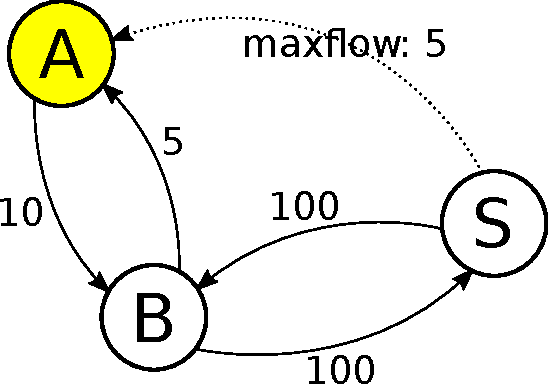
\includegraphics[width=0.3\textwidth]{bartercast}
  \caption{Subjective graph of $A$. The numbers are the amout of data transfered,
    they can be seen as the capacity in the context of the maximum flow
    problem.}
  \label{fig:bartercast}
\end{figure}

BarterCast does not prevent the Sybil attack by itself. Because attackers can
first upload a lot of data to obtain a good reputation in the network. If the
attacker now creates Sybils and false report of the Sybils saying that they
uploaded a lot. Then the peers who have interacted with the attacker will be
tricked to think that the Sybils also have a high reputation. To fix this
problem, Delaviz et el. created SybilRes\cite{delaviz2012sybilres}. The main
idea is the following. Suppose there are two peers $A$ and $B$ who are sharing
data. If $A$ is uploading (represented by an outgoing edge) to $B$, then it
decreases the weight of the incoming edge from $B$. Vice versa, the weight is
increased for the outgoing edge when $A$ is downloading. The rate of change
depends on the capacities of the edges and the amout of data transferred after
computing the reputation. Using the definition in \autoref{fig:attack-edge}, the
attacker cannot built up reputation for its Sybils by uploading to peers in the
honest region beforehand, it is now forced to keep on uploading to keep its
Sybil's reputation which is a much more desirable behaviour.

Seuken et al. provided a formal model of BarterCast. They found that BarterCast
is vulnerable to misreporting and proposed a solution called the DropEdge
mechanism\cite{seuken2011sybil, seuken2014sybil}. DropEdge, like the name
implies, drops some edges in the subjective graph that satisfies the following
constraints. Suppose peer $A$ wishes to download from peers in set $C$ (the
choice set). Then any reports received by $A$ from $p \in C$ is dropped. Also,
edges with both end points in $C$ are also dropped from $A$'s subjective graph.
Intuitively, peers in $C$ cannot misreport their contribution. The authors
formally prove this property in their work. They also prove that it is robust
against weakly benefician Sybils, that is Sybils that do not perform actual work
for honest peers.

SumUp\cite{tran2009sybil} is a defence mechanism specific for the vote
aggregation problem. For example, in social news aggregation websites such as
Reddit, users vote on the submitted content to determine its ranking; the
problem occurs when Sybils can out-vote honest users. It is a centralised
approach that fits the architecture of most websites that perform vote
aggregation. SumUp consist of three stages. Firstly, pruning is performed to
limit the number of incoming edges of every node, this is to reduce the number
of attack edges available and reduce the computational cost in later stages, the
threshold is a system parameter. Secondly, it uses a ticket source (the central
component) distributes tickets in a breadth-first search manner equally to its
neighbours, every node keeps one ticket and distributes the remaining tickets
the same way. The number of tickets distributed across an edge plus one is the
capacity of the edge. Effectively, edges closer to the ticket source have a high
capacity. This idea keeps the capacities in the Sybil region low so that they do
not have a large influence on the outcome. Finally, the maximum flow is computed
where the source is simply the ticket source and the sink is an imaginary node
with edges of capacity one that is connected to every voter. SumUp offers a
better guarantee than SybilLimit where it only accepts $1 + o(n)$ votes per
attack edge. An improved version of SumUp - GateKeeper is discussed in
\autoref{sec:random-walk}.

TODO diagram for ticket distribution?

Conversely, maximum flow is dual to minimum cut, so the problem of finding Sybil
can also be formulated as finding sparse cuts\footnote{The sparse cut problem is
  to find a partition such that the ratio between the number in the cut and the
  number of vertices in the smaller partition is minimised. This problem is
  related to minimum cut.}. Kurve and Kesidis devised an algorithm for finding
sparse cuts to detect Sybils\cite{kurve2011sybil}. Unlike the aforementioned
techniques, it relies on the presence of trusted nodes.

\subsection{Random Walk Based Techniques}\label{sec:random-walk}
Another family, possibly the largest, Sybil defence mechanism is based on random
walks. The key assumptions in these techniques is that the honest region is
\emph{fast mixing}\footnote{In a graph, if a random walk of length $O(\log{N})$
  reaches a stationary distribution of nodes, then the graph is fast mixing.},
and the attack edges are difficult to form and are independent of the number of
Sybils. The first defence mechanism is SybilGuard\cite{yu2006sybilguard},
created by Yu et el. SybilLimit\cite{yu2008sybillimit} is the continuation of
SybilGuard and it is an improvement on many fronts while keeping the same or
better guarantees as SybilGuard. In this section we focus on SybilLimit plus
other random walk based techniques.

Before explaining SybilLimit, we define the term \emph{random route}. Random
route is a modified form of a random walk. In random walk, a outgoing edge is
selected uniformly at random on every hop of the walk. In random route, every
node maintains a static routing table that contains a uniformly random
one-to-one mapping between incoming edges and outgoing edges, initialised at
start-up. Thus the route is determined by the tables on every node. An important
property of random route is that if two routes enter the same edge, then they
will always exit at the same edge, so their route after exiting will be exactly
the same. The number of hops for a random route (the mixing time) should be just
right, so that the fast mixing property is achieved only in the honest region.

In SybilLimit, every honest node acts as a verifier $V$ and initially treats all
other nodes as suspects $S$. The verification process begins by performing
multiple independent random routes by each party. $V$ labels $S$ as an honest
node if and only if they share at least one tail (the final edge in the route).
For each tail of $V$, there is a quota for the number of node that it labels.
The authors prove that SybilLimit bounds the number of accepted Sybils (false
positives) at $O(\log{n})$, an improvement from $O(\sqrt{n} \log{n})$ of
SybilGuard.

Let us consider the following three scenarios to intuitively show why SybilLimit
works. Suppose $S$ is not a Sybil, and if $V$ and $S$ perform enough random
routes, each with enough hops for fast mixing, then due to the Birthday Paradox,
$S$ and $V$ will have an intersecting tail with high probability. Next, suppose
some of the tails of $V$ are in the Sybil region so they may intersect with a
large number of Sybils, but crossing the attack edges is improbable and
accepting a lot of Sybils is also difficult due to the aforementioned quota
mechanism, thus $V$ has a small probability of accepting a large number of
Sybils. Finally, consider there is only one attack edge and suppose a Sybil has
tails in the honest region, due to the random route property, the route of the
Sybils in the honest region will be exactly the same, so accepting the Sybils in
this scenario is also low due to the quota mechanism.

TODO create a diagram for SybilLimit

SybilGuard and SybilLimit inspired many other defence mechanisms.
SybilInfer\cite{danezis2009sybilinfer} assumes trusted nodes, which create
traces by doing random walks in the graph. Based on the traces, a probability
model that descries the likelihood a trace $T$ was generated by a specific set
of honest nodes $X$, i.e. $\Pr[ T | X = \text{honest}]$. Then using Bayesian
inference, $\Pr[ X = \text{honest}| T ]$ can be computed, that is effectively
assigning a ``score'' to every node. Sybil are the nodes with a low ``score''.
SybilInfer outperforms SybilLimit regarding the number of false positives, but
its drawbacks are its high computational cost and reliance on trusted nodes.

Viswanath et al. realised many of the aforementioned mechanisms in this section
is in fact performing local community detection (i.e. detecting clusters of
nodes) which is a more developed field\cite{viswanath2010analysis}. The authors
also argue that social graphs are not always fast mixing, which may result in
poor results for techniques that uses the fast mixing assumption. Using
synthetic social graphs, the authors show that applying Mislove's
algorithm\cite{mislove2010you} achieve similar results as SybilLimit and
SybilInfer. But using a Facebook social graph, Mislove's algorithm performs
better.

SybilDefender\cite{wei2012sybildefender} can be seen as a two step process. It
assumes the size of the Sybil region is smaller than the honest region and the
nodes in the Sybil region are well connected. The first step is to perform
random walk to detect Sybils. The second step is to detect a complete Sybil
region around the detected Sybils. The algorithm in the second step employs
\emph{partial} random walk, where the random walk is not allowed to traverse the
same node more than once. The property of the partial random walks is that they
are likely to ``die'' (all the neighbour nodes have already been traversed) upon
reaching the edge of the Sybil region, thus they are likely to stay in the Sybil
region. The Sybil region is detected by examining the nodes traversed by the
partial random walk.

% how does SybilDefender guarantee that the Sybils actually perform the random
% walk correctly in the second step?

SybilRank, in contrast of the aforementioned techniques, is designed to be
integrated with real-world OSN and is deployed on Tuenti (an OSN with 11 million
users)\cite{cao2012aiding}. SybilRank uses short random walks that begins on
trusted nodes in the honest region. The trusted nodes is choosen manually, this
allows SybilRank to adapt to different graph structures. A novelty in SybilRank
is that it uses power iterations, an efficient technique for computing the
landing probability of random walks. Intuitively, the probability decreases for
nodes that are far away from the trusted nodes, especially for nodes in the
Sybil region. The probabilities are normalised by the degree of the node and
then ranked. The potential Sybils are the nodes that are under a some threshold.
Finally, various actions can be performed to to verify the potential Sybils,
e.g. using CAPTCHA puzzles.

SybilShield\cite{shi2013sybilshield} makes use of multiple communities. It
begins the same way as SybilGuard/SybilLimit, i.e. $V$ performs random route to
determine whether suspect $S$ is a Sybil. But to reduce the possibility that $S$
is in fact an honest node but labeled as a Sybil, $V$ searches for agents $A$
that are from another community (also using random route). $A$ performs the same
random route algorithm and decides whether $S$ is actually a Sybil and then
relay the information to $V$. If a large majority of $A$ say $S$ is honest, then
$V$ knows that it has made a mistake, otherwise $S$ is indeed a Sybil.

TODO make figure of multiple communities for SybilShield

GateKeeper\cite{tran2011optimal} combines ideas from SumUp (discussed in
\autoref{sec:network-flow}) and SybilLimit. GateKeeper assumes a admission
controller that is honest, the admission controller performs random walks to
select $n$ ticket sources. The ticket sources act the same way as SumUp where it
distributes ticket in a breadth-first search manner. For a node to be labeled
honest, it must obtain $fn$ tickets, where $f$ is a system parameter (0.2 is
shown to be a good value experimentally). This idea works becauses if the ticket
sources are evenly distributed and Sybils ony have a few attack edges, then it
is unlikely that they will receive a large number of tickets.

% Whanau\cite{lesniewski2010whanau}
% ReDS\cite{akavipat2014reds} suggests to use sybilimit or sybilinfer

\subsection{Distrust Relationships}
Ostra\cite{mislove2008ostra}
VoteTrust\cite{xue2013votetrust}

\subsection{Content Driven}
\cite{chatterjee2008robust}

\subsection{Reputation Transfer}
Trust-transfer\cite{seigneur2005trust}

\subsection{Cryptography Based Techniques?}
Secure-Overlay\cite{lua2007securing} - ID crypto and SSS
Privacy-preserving\cite{schaub2016trustless} - blockchain?
Proof-of-stake\cite{dennis2016rep}

\subsection{Other}
Parental control\cite{tehale2012parental} - uses parents to ``observe'' find suspects, only for detection, requires a sybil-proof reputation scheme
DSybil\cite{yu2009dsybil} - recommendation system, need historical data
Symon\cite{jyothi2009symon} - pair peers together, likelihood for both to be sybils is low, the pair monitor each other to prevent attacks
XRep 02\cite{damiani2002reputation} IP check, and checks digest, uses existing P2P systems like Gnutella

\subsection{Unsorted?}

Beth and PGP limits Sybil attack to some extent by using social graphs
Beth 94\cite{beth1994valuation}
PGP (Zimmermann) 95\cite{zimmermann1995official}

Yu 00\cite{yu2000social}
% CORE 02\cite{michiardi2002core} % MANETs
Lee 03\cite{lee2003cooperative} - uses flooding, might not be scalable, only talks about DoS
% Buchegger 04 - MANETs
% Xiong 03\cite{xiong2003reputation} % also PeerTrust?
Marti 04\cite{marti2004limited}
ARA 05\cite{ham2005ara} - no mention of sybil, prevents freeriding, prevents short-term abuse because reputation increases gradually
FuzzyTrust Song 05\cite{song2005trusted} - uses fuzzy logic
P2PRep/Fuzzy 06\cite{aringhieri2006fuzzy} - also fuzzy, does not prevent generation of false rumors
Xiong 05\cite{xiong2007countering} - no mention of sybil, but tries to mitigate false information
PowerTrust 06\cite{zhou2007powertrust} - uses ``power nodes'' (from power-law), no mention of sybil, some defence against colluders
% Li 07 - MANETs

Histos and Sopras\cite{zacharia2000collaborative}, doesn't really have structure?
Beta\cite{jsang2002beta}
% Confidant\cite{buchegger2002performance} MANETs
Gupta et al.\cite{gupta2003reputation}

PeerTrust\cite{xiong2004peertrust} - DHT, used P-GRID source code, has credibility rating

PerContRep\cite{yan2014percontrep}


\subsection{Does not handle Sybil-attack?}
TrustMe\cite{singh2003trustme} is a reputation that focuses on anonymity, no mention of sybil attack

H-Trust\cite{zhao2009htrust} does not mention sybil

Coner et al.\cite{conner2009trust} assumes clients cannot perform sybil attack

TrustGuard 05\cite{srivatsa2005trustguard} - assumes it is built on secure overlay networks (sybil-proof networks)

Scrivener 05\cite{nandi2005scrivener} - assumes ID cannot be created and discarded

%%% Local Variables:
%%% mode: latex
%%% TeX-master: "main"
%%% End:
